\documentclass[cjk,slidestop,compress,mathserif,blue]{beamer}
%dvipdfm选项是关键,否则编译统统通不过
%beamer的颜色选项定义的是导航条和标题的颜色(即关键词structure的颜色)

%%%%%%%%%%%%%%%%仅限于XeTeX可使用的宏包%%%%%%%%%%%%%%%%%%%%%%%%%%%%
\usepackage{fontspec,xunicode,xltxtra,beamerthemesplit}
%\usepackage{beamerthemesplit}
\usepackage{handoutWithNotes}		%(讲义)在打印PPT的时候会留出给每一页做注释的部分
\usepackage{xeCJK}
\setCJKmainfont[BoldFont=黑体, ItalicFont=楷体, BoldItalicFont=仿宋]{黑体}
%\setsansfont[Mapping=tex-text]{Adobe 黑体 Std}
%如果装了Adobe Acrobat,可在font.conf中配置Adobe字体的路径以使用其中文字体
%也可直接使用系统中的中文字体如SimSun,SimHei,微软雅黑 等
%原来beamer用的字体是sans family;注意Mapping的大小写,不能写错

\usepackage{listings} 
\lstset{language=Matlab}%代码语言使用的是matlab 
\lstset{breaklines}%自动将长的代码行换行排版 
\lstset{extendedchars=false}%解决代码跨页时,章节标\dots

%%%%%%%%   确定标题和导航条结构的框架     %%%%%%%%%%%%
\usepackage{beamerthemeshadow}                       %
%\usepackage{beamerthemeclassic}%导航条色与背景色一致%
%%%%%%%%%%%%%%%%%%%%%%%%%%%%%%%%%%%%%%%%%%%%%%%%%%%%%%
\setbeamerfont{roman title}{size={}}
%\usepackage{CJK} % CJK 中文支持                                  %
\usepackage{amsmath,amsthm,amsfonts,amssymb,bm}
\usepackage{bbding}
\usepackage{mathrsfs}
\usepackage{xcolor}                                        %使用默认允许使用颜色
\usepackage{hyperref} 
\usepackage{graphicx}
\usepackage{subfigure}           %图片跨页
\usepackage{animate}		 %插入动画
\usepackage{caption}
\captionsetup{font=footnotesize}

\usepackage{multirow}

\usepackage[dvipdfmx]{movie15_dvipdfmx} %插入视频
%\usepackage{handoutWithNotes}		%(讲义)在打印PPT的时候会留出给每一页做注释的部分
%\pgfpagesuselayout{1 on 1 with notes landscape}[a4paper,border shrink=5mm]

%\usepackage[numbers,sort&compress]{natbib} %紧密排列             %
\usepackage[sectionbib]{chapterbib}        %每章节单独参考文献   %
\usepackage{hypernat}                                                                         %
%\usepackage[dvipdfm,bookmarksopen=true,pdfstartview=FitH,CJKbookmarks]{hyperref}		%
\hypersetup{bookmarksnumbered,colorlinks,linkcolor=brown,citecolor=blue,urlcolor=red}         %
%参考文献含有超链接引用时需要下列宏包,注意与natbib有冲突        %
%\usepackage[dvipdfm]{hyperref}                                  %
%\usepackage{hypernat}                                           %
\newcommand{\upcite}[1]{\hspace{0ex}\textsuperscript{\cite{#1}}} %

%\usepackage{marvosym} %插入各种符号

%\useoutertheme{smoothbars}
\useinnertheme[shadow=true]{rounded}
\usetheme{Berkeley}                                          %主题式样
%\usetheme{Luebeck}

\usecolortheme{lily}                                        %颜色主题式样

\usefonttheme{professionalfonts}                           %字体主题样式宏包

%\beamertemplatetransparentcoveredhigh                      %使所有被隐藏的文本高度透明
\beamertemplatetransparentcovereddynamicmedium             %使所有被隐藏的文本完全透明,动态,动态的范围很小
\mode<presentation>
%\beamersetaveragebackground{gray}                          %设置背景颜色(单一色) 
\beamertemplateshadingbackground{green!10}{red!5}         %设置背景颜色(渐变色)

%i放置单位logo
%\logo{
\includegraphics[width=1.6cm,height=0.35cm]{Figures/BCC_logo-1.png}}	%简单设置logo

%\pgfdeclareimage[width=3.5cm]{logoname}{Figures/BCC_logo-1.png}		%logo置于左侧微调
%\logo{\pgfuseimage{logoname}{\vspace{0.2cm}\hspace*{-2.0cm}}}

%在指定位置精确放置logo
\usepackage{tikz}
\usepackage{beamerfoils}
\usepackage{pgf}
\logo{\pgfputat{\pgfxy(11.68,0.15)}{
\includegraphics[height=1.01cm,viewport=0 0 140 120,clip]{Figures/BCC_logo-1.png}}\pgfputat{\pgfxy(10.502,-0.218)}{
\includegraphics[height=0.369cm,viewport=140 0 540 120,clip]{Figures/BCC_logo-1.png}}}
%\logo{\pgfputat{\pgfxy(11.68,0.15)}{
\includegraphics[height=0.95cm,viewport=0 0 510 360,clip]{Figures/Logo_Gainstrong.png}}\pgfputat{\pgfxy(10.333,-0.195)}{
\includegraphics[height=0.35cm,viewport=530 70 1100 218,clip]{Figures/Logo_Gainstrong.png}}}
%\logo{\pgfputat{\pgfxy(10.28,0.00)}{
\includegraphics[height=0.95cm,viewport=0 0 1100 360,clip]{Figures/Logo_Gainstrong.png}}}
%\logo{\pgfputat{\pgfxy(11.68,0.15)}{
\includegraphics[height=0.95cm,viewport=0 0 510 360,clip]{Figures/Logo_Gainstrong.png}}\pgfputat{\pgfxy(10.333,-0.195)}{
\includegraphics[height=0.35cm,viewport=530 70 1100 218,clip]{Figures/Logo_Gainstrong.png}}}
%\MyLogo{
%	\pgfputat{\pgfxy(-50,-50)}{\pgfbox[right,base]{
\includegraphics[height=1cm]{Figures/BCC_logo-1.png}}}

%logo作为背景放置
%\setbeamertemplate{background}{
%	\pgfputat{\pgfxy(6.5,-0.5)}{\pgfbox[left,top]{\pgfimage[height=1.1cm]{Figures/BCC_logo-1.png}}}}

%\logo{}									%不显示logo

\begin{document}
%\begin{CJK*}{GBK}{song}
%\begin{CJK*}{GBK}{kai}
%beamer下不能用\songyi、\zihao等命令!
%\graphicspath{Figures/}

%-------------------------------PPT Title-------------------------------------
\title{高通量材料自动流程计算软件框架:\\\rm{MP}与\rm{ASE}}
%-----------------------------------------------------------------------------

%----------------------------Author & Date------------------------------------
\author[\textrm{Jun\_Jiang}]{姜\;\;骏\inst{}} %[]{} (optional, use only with lots of authors)
% - Give the names in the same order as the appear in the paper.
% - Use the \inst{?} command only if the authors have different
%   affiliation.
\institute[BCC]{\inst{}%
 \vskip -30pt 北京市计算中心}
\date[\today] % (optional, should be abbreviation of conference name)
{	{\fontsize{6.2pt}{4.2pt}\selectfont{\textcolor{blue}{E-mail:~}\url{jiangjun@bcc.ac.cn}}}
\vskip 35 pt {\fontsize{8.2pt}{6.2pt}\selectfont{2019.12.27}}
\vskip 5 pt {\fontsize{8.2pt}{6.2pt}\selectfont{国家超级计算济南中心}}}

% - Either use conference name or its abbreviation
% - Not really information to the audience, more for people (including
%   yourself) who are reading the slides online

\subject{}
% This is only inserted into the PDF information catalog. Can be left
% out.
\frame
{
%	\frametitle{\fontsize{9.5pt}{5.2pt}\selectfont{\textcolor{orange}{“高通量并发式材料计算算法与软件”年度检查}}}
\titlepage
}
%-----------------------------------------------------------------------------

%------------------------------------------------------------------------------列出全文 outline ---------------------------------------------------------------------------------
\section*{}
\frame[allowframebreaks]
{
  \frametitle{Outline}
%  \frametitle{\textcolor{mycolor}{\secname}}
  \tableofcontents%[current,currentsection,currentsubsection]
}
%在每个section之前列出全部Outline
%类似的在每个subsection之前列出全部Outline是\AtBeginSubsection[]
\AtBeginSection[]
{
  \frame<handout:0>
  {
    \frametitle{Outline}
%全部Outline中,本部分加亮
    \tableofcontents[current,currentsection]
  }
}

%------------------------------------------------------------------------------PPT main Body------------------------------------------------------------------------------------
\small
\section{材料电子结构计算软件的基本结构}       %Bookmark
\frame
{
	\frametitle{材料基因工程的基本思想}
\begin{figure}[h!]
\centering
\vspace*{-0.2in}
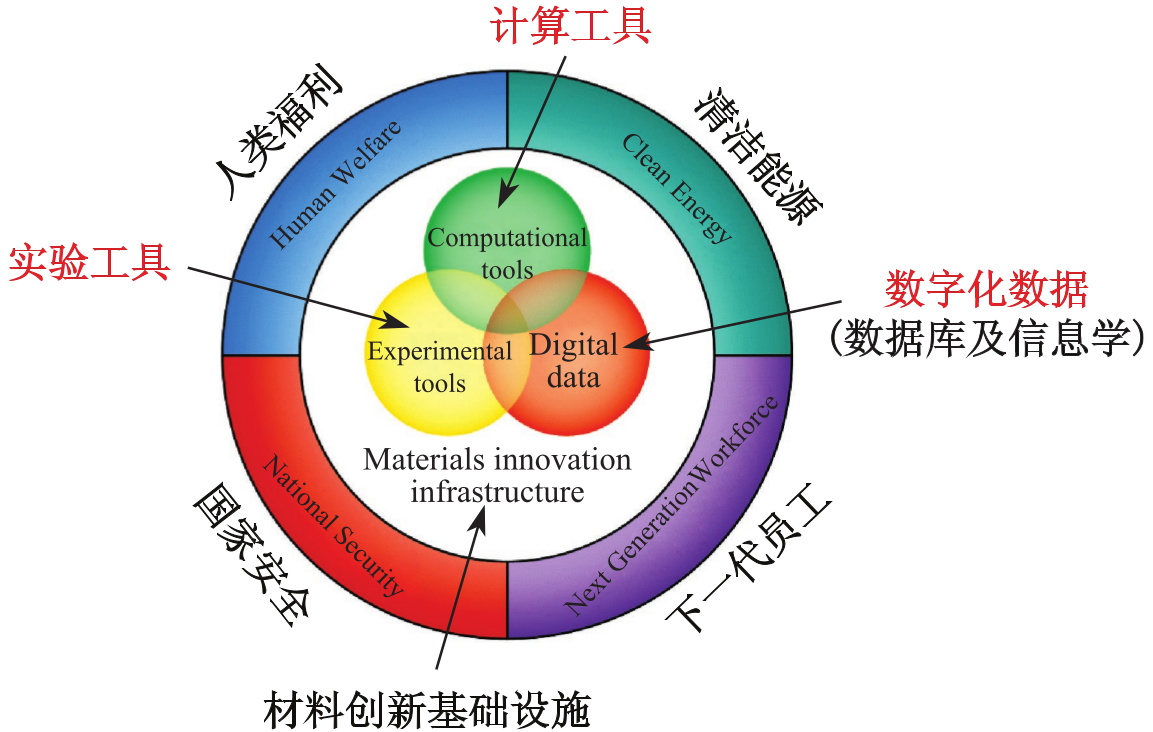
\includegraphics[width=0.6\textwidth]{Figures/Mat_Geno_Ene-1.png}
\vskip 0.10in
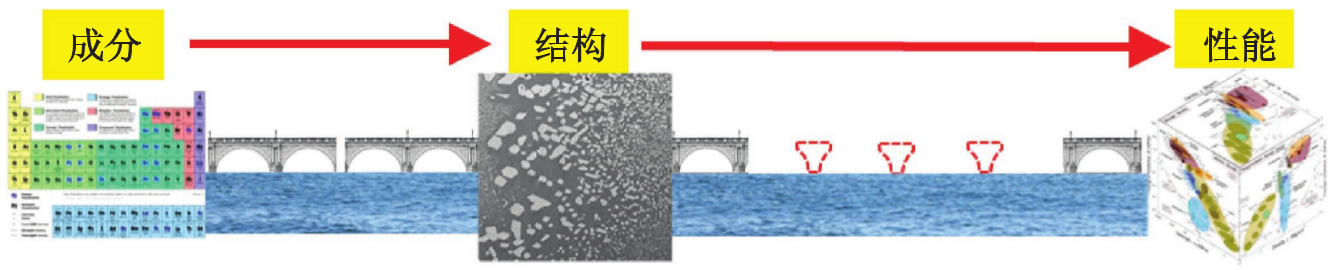
\includegraphics[height=0.85in]{Figures/Mat_Geno_Ene-3.png}
\label{Mater_Genome}
\end{figure}
}

\frame
{
	\frametitle{材料模拟的基本思想}
\begin{figure}[h!]
\vspace*{-0.25in}
\centering
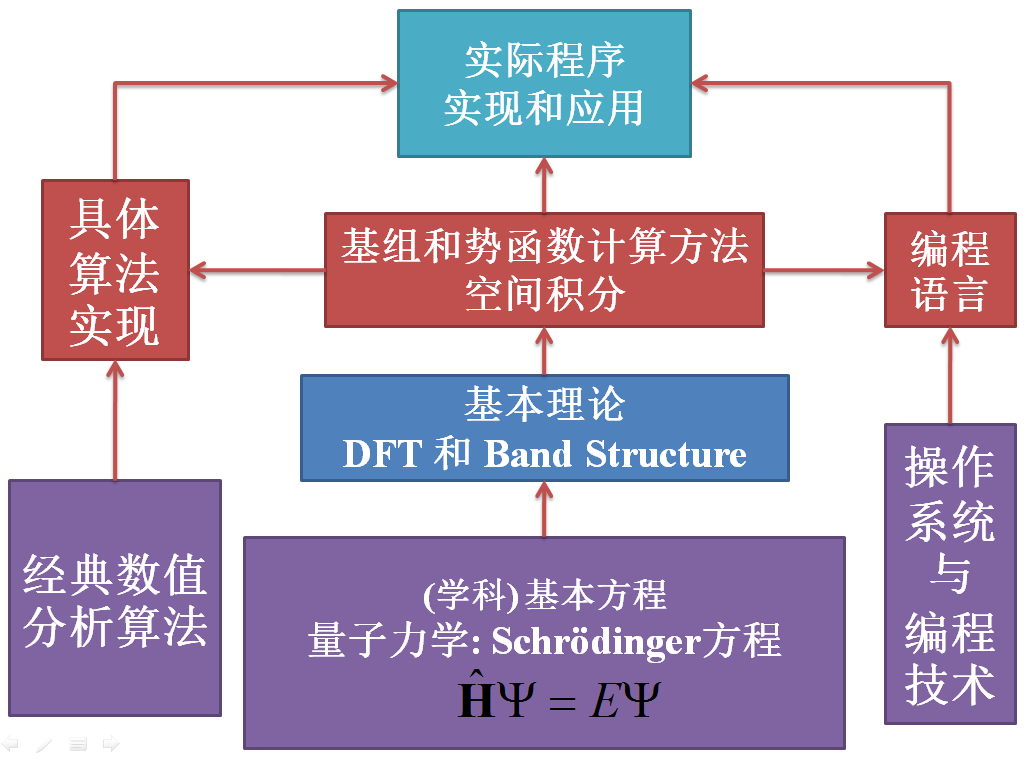
\includegraphics[height=2.80in,width=4.95in,viewport=5 3 1250 780,clip]{Figures/Method_Procedure.png}
%\caption{\small \textrm{Pseudopotential for metallic sodium, based on the empty core model and screened by the Thomas-Fermi dielectric function.}}%(与文献\cite{EPJB33-47_2003}图1对比)
\label{Method-Procedure}
\end{figure}
}

\frame
{
	\frametitle{第一原理计算框架:~\textrm{DFT-SCF}}
\begin{figure}[h!]
\centering
\vspace*{-0.25in}
\hspace*{-0.80in}
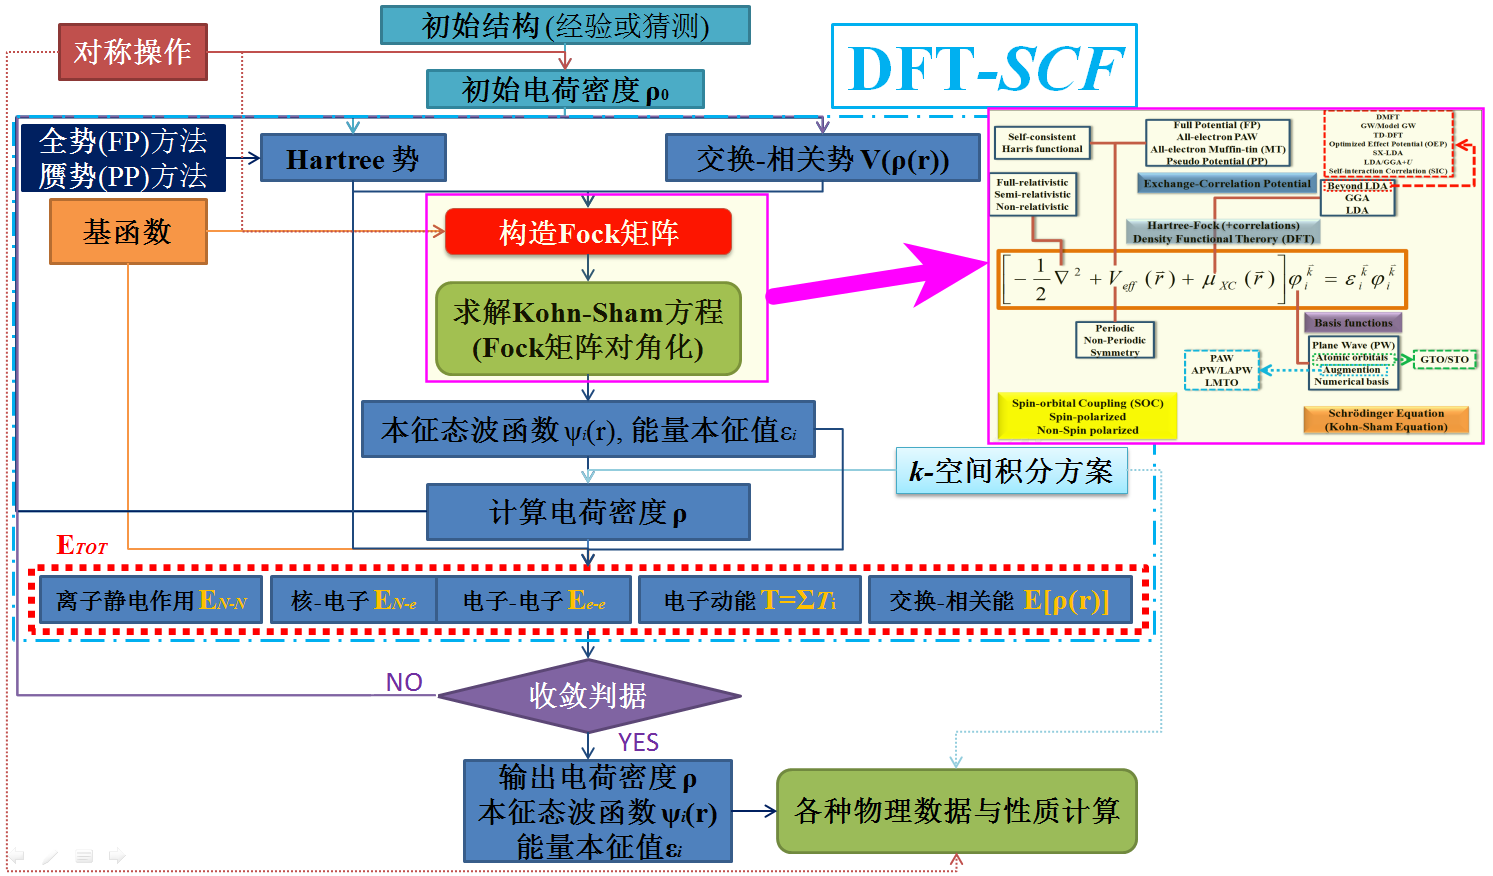
\includegraphics[height=2.80in,width=4.95in,viewport=5 3 1490 870,clip]{Figures/DFT-SCF_2.png}
%\caption{\small \textrm{Pseudopotential for metallic sodium, based on the empty core model and screened by the Thomas-Fermi dielectric function.}}%(与文献\cite{EPJB33-47_2003}图1对比)
\label{Pseudo-NC}
\end{figure}
}

\section{材料计算平台开发现状}     %Bookmark
\frame
{
	\frametitle{国内已有的计算平台:~MatCloud}
\begin{figure}[h!]:
\centering
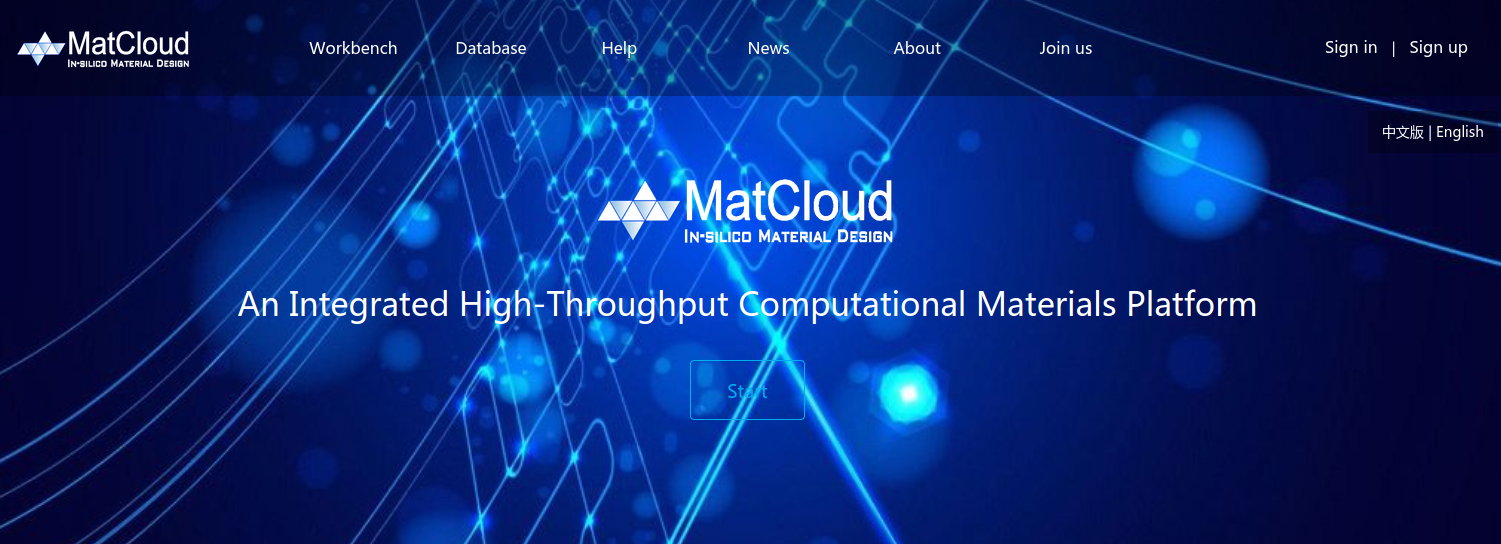
\includegraphics[height=1.57in,width=4.95in,viewport=0 0 1800 550,clip]{Figures/Matcloud-login.png}
\caption{\fontsize{7.2pt}{4.2pt}\selectfont{中科院计算机网络信息中心~杨小渝研究员~团队~开发}\upcite{CMS146-319_2018,url_Matcloud}}%
\label{Auto_Flow_Platform-2}
\end{figure}
}

\frame
{
	\frametitle{国外已有的计算平台}
\begin{figure}[h!]
\centering
\vspace{-15.5pt}
\subfigure[\fontsize{7.5pt}{6.2pt}\selectfont{\textrm{Auto-FLOW (AFLOW)}\upcite{CMS58-227_2012}}]{
\label{AFLOW_data_flow}
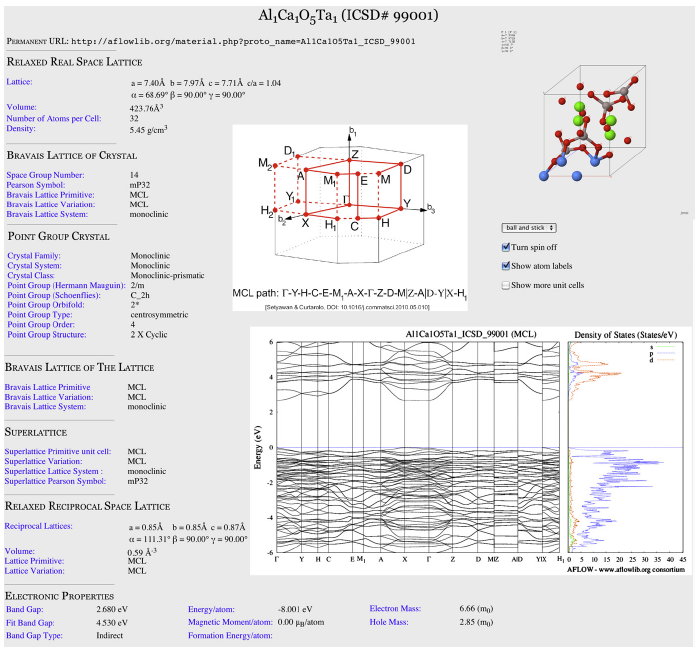
\includegraphics[height=1.2in,width=1.6in,viewport=0 0 720 660,clip]{Figures/AFLOW_database.png}}
\subfigure[\fontsize{7.5pt}{6.2pt}\selectfont{\textrm{Material Project (MP)}\upcite{CMS97-209_2015}}]{
\label{MP_commp_infrastructure}
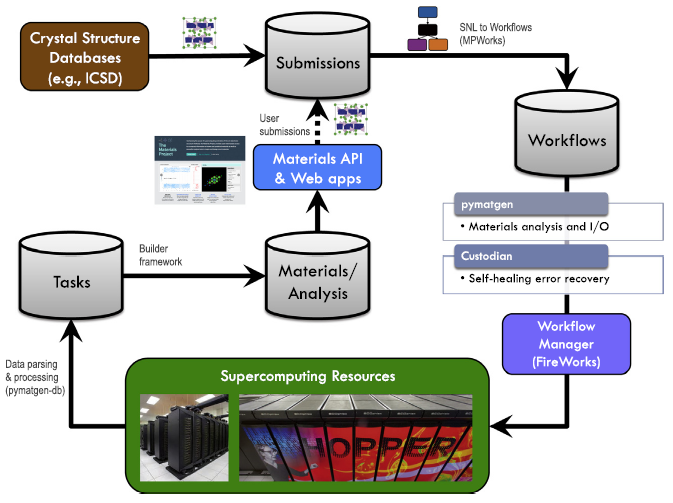
\includegraphics[height=1.2in,width=1.7in,viewport=0 0 670 530,clip]{Figures/MP_comp_infrastructure.png}}
\subfigure[\fontsize{3.5pt}{3.2pt}\selectfont{\textrm{Quantum Materials Informatics Project (QMIP)}\upcite{url_QMIP}}]{
\label{QMIP_Shame}
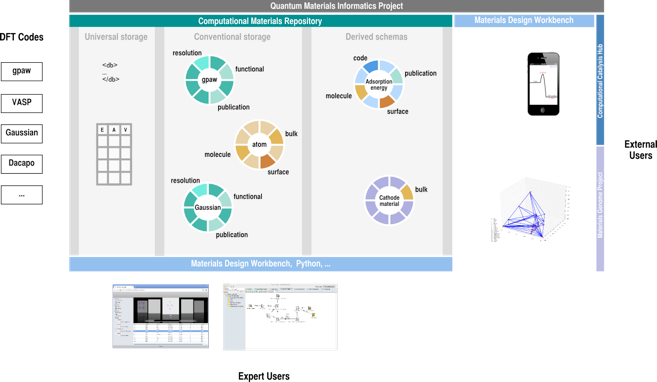
\includegraphics[height=1.2in,width=1.7in,viewport=0 0 670 420,clip]{Figures/QMIP_shame.png}}
\subfigure[\fontsize{6.5pt}{5.2pt}\selectfont{\textrm{Clean Energy Project (CEP)}\upcite{JPCL2-2241_2011}}]{
\label{CEP_structure_flow}
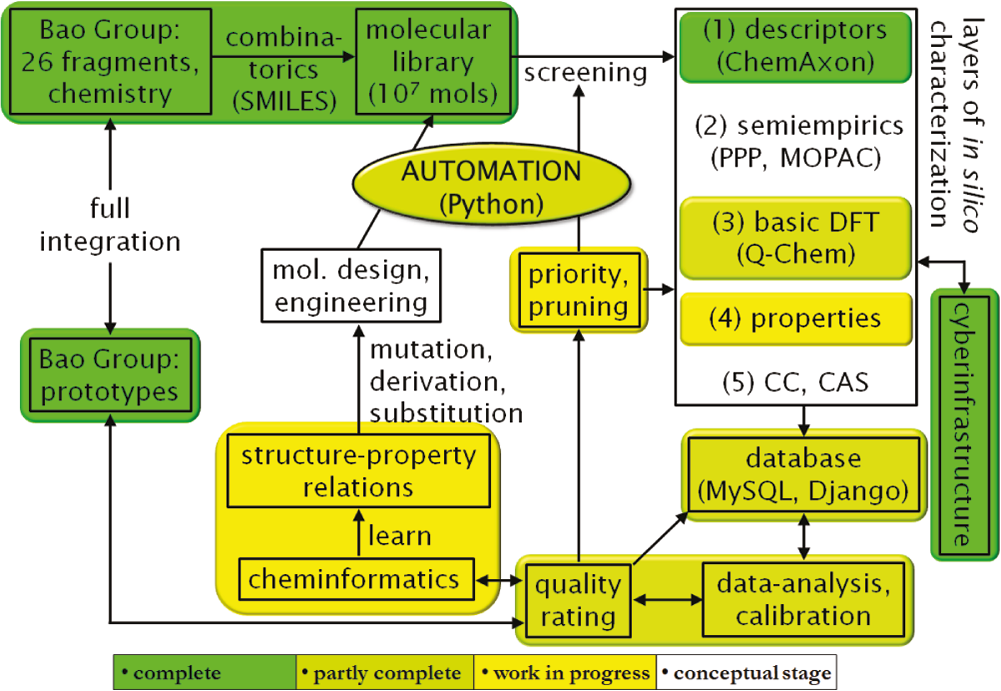
\includegraphics[height=1.2in,width=1.6in,viewport=0 0 1020 730,clip]{Figures/CEP_structure_flow.png}}
%\caption{}%
\label{Auto_Flow_Platform-1}
\end{figure}
}

\frame
{
	\frametitle{\textrm{ASE}:~接口丰富的适应性计算平台}
\begin{figure}[h!]
\centering
\vspace*{-0.2in}
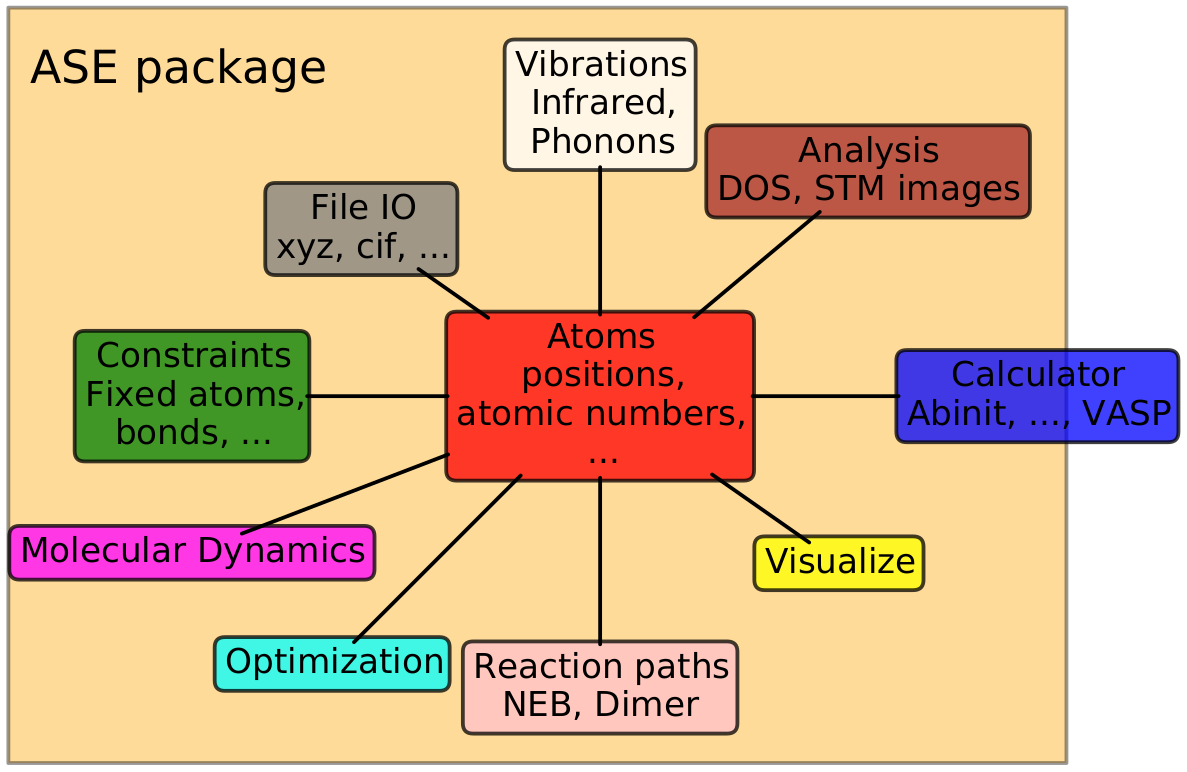
\includegraphics[height=2.1in,width=3.2in,viewport=0 0 1208 830,clip]{Figures/ASE_Python_lib.png}
\caption{\fontsize{7.2pt}{4.2pt}\selectfont{\textrm{ASE:~a Python library for working with atoms.}}}%
\label{Logo_ASE_lib}
\end{figure} 
}

\frame
{
	\frametitle{现有高通量计算平台概览}
\begin{table}[!h]
\tabcolsep 0pt \vspace*{-12pt}
%\caption{}
\label{Table-Cost}
\begin{minipage}{0.85\textwidth}
%\begin{center}
\centering
\def\temptablewidth{1.1\textwidth}
\renewcommand\arraystretch{0.8} %表格宽度控制(普通表格宽度的两倍)
\rule{\temptablewidth}{1pt}
\begin{tabular*} {\temptablewidth}{@{\extracolsep{\fill}}c@{\extracolsep{\fill}}c@{\extracolsep{\fill}}c@{\extracolsep{\fill}}c@{\extracolsep{\fill}}c@{\extracolsep{\fill}}c@{\extracolsep{\fill}}c}
%-------------------------------------------------------------------------------------------------------------------------
	&\multirow{2}{*}{\fontsize{7.2pt}{5.2pt}\selectfont{编程语言}}	&\fontsize{7.2pt}{5.2pt}\selectfont{建模} &\multicolumn{2}{|c|}{\fontsize{6.2pt}{5.2pt}\selectfont{任务提交与管理}} &\multirow{2}{*}{\fontsize{7.2pt}{5.2pt}\selectfont{后处理}} &\multirow{2}{*}{\fontsize{6.2pt}{5.2pt}\selectfont{数据组织管理}} \\\cline{4-5}
	&	&\fontsize{7.2pt}{5.2pt}\selectfont{功能} &\multicolumn{1}{|l}{\fontsize{7.2pt}{5.2pt}\selectfont{软件接口}} &\multicolumn{1}{r|}{\fontsize{7.2pt}{5.2pt}\selectfont{运行容错}} & & \\\hline
	\fontsize{7.2pt}{5.2pt}\selectfont{{AFLOW}} &\fontsize{7.2pt}{5.2pt}\selectfont{C++} &\checkmark &\triangle &\FiveStarOpen &\FiveStarOpen &\fontsize{7.2pt}{5.2pt}\selectfont{{Django}} \\
	\fontsize{7.2pt}{5.2pt}\selectfont{{MP}} &\fontsize{7.2pt}{5.2pt}\selectfont{Python} &\checkmark &\checkmark &\FiveStarOpen &\FiveStarOpen &\fontsize{7.2pt}{5.2pt}\selectfont{{MongoDB}} \\
	\multirow{2}{*}{\fontsize{7.2pt}{5.2pt}\selectfont{{QMIP}}} &\fontsize{7.2pt}{5.2pt}\selectfont{JavaScript/SVG} &\multirow{2}{*}{\checkmark} &\multirow{2}{*}{\checkmark} &\multirow{2}{*}{--} &\multirow{2}{*}{\checkmark} &\multirow{2}{*}{--} \\
	&\fontsize{7.2pt}{5.2pt}\selectfont{+html/Python} & & & & & \\
	\fontsize{7.2pt}{5.2pt}\selectfont{{CEP}} &\fontsize{7.2pt}{5.2pt}\selectfont{Python} &\checkmark &\checkmark &-- &\checkmark &\fontsize{7.2pt}{5.2pt}\selectfont{{Django/MySQL}} \\
	\fontsize{7.2pt}{5.2pt}\selectfont{{ASE}} &\fontsize{7.2pt}{5.2pt}\selectfont{Python} &\FiveStarOpen &\FiveStarOpen &-- &\triangle &-- \\
	\multirow{2}{*}{\fontsize{7.2pt}{5.2pt}\selectfont{{MatCloud}}} &\fontsize{7.2pt}{5.2pt}\selectfont{JavaScript} &\multirow{2}{*}{\checkmark} &\multirow{2}{*}{\triangle} &\multirow{2}{*}{\checkmark} &\multirow{2}{*}{\checkmark} &\multirow{2}{*}{\fontsize{7.2pt}{5.2pt}\selectfont{{MongoDB}}} \\
	&\fontsize{7.2pt}{5.2pt}\selectfont{+.NETCore} & & & & &
\end{tabular*}
\rule{\temptablewidth}{1pt}
\end{minipage}
%\vskip -15pt
\fontsize{7.2pt}{5.2pt}\selectfont{
\begin{description}
	\item[\FiveStarOpen]~该功能较突出
	\item[\checkmark]~该功能基本满足需求
	\item[\triangle]~该功能存在不足
\end{description}}
%\end{center}
\end{table}
}

\frame
{
	\frametitle{\textrm{计算平台的功能和总体架构}}
\begin{figure}[h!]
\centering
\hspace*{-0.2in}
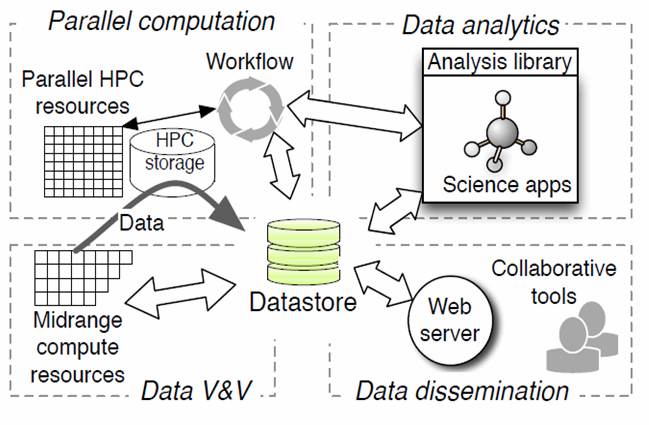
\includegraphics[height=1.25in,width=1.95in,viewport=0 0 670 460,clip]{Figures/Parallel_computation.png}
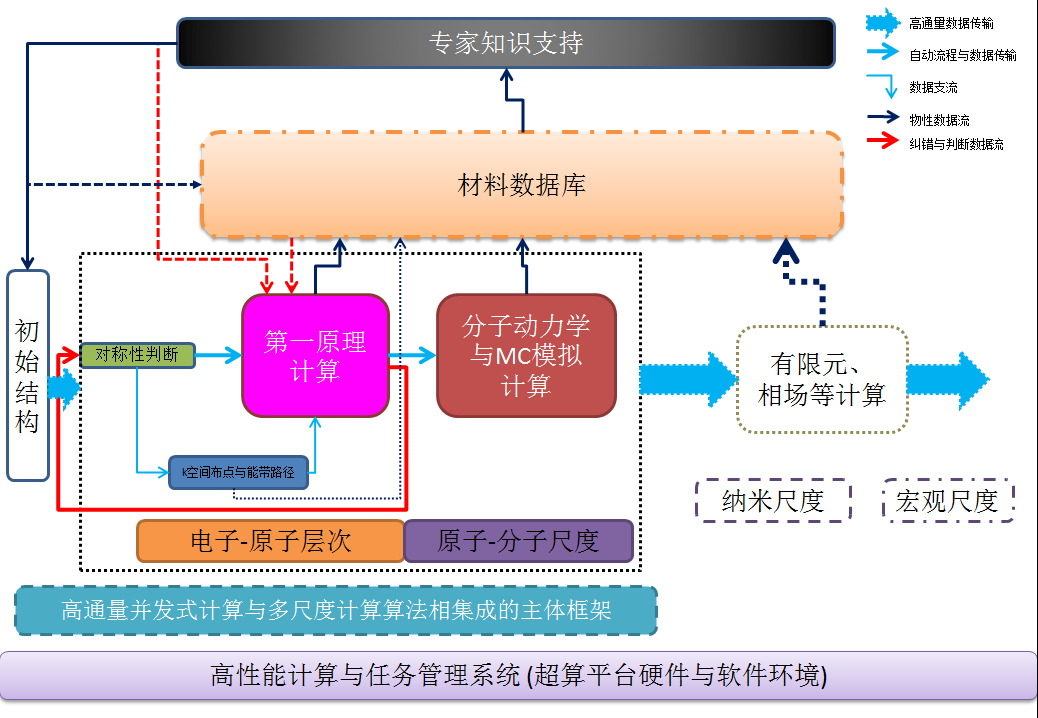
\includegraphics[height=1.6in,width=2.4in,viewport=0 0 1038 730,clip]{Figures/Auto_Flow.png}
\caption{\fontsize{7.2pt}{4.2pt}\selectfont{\textrm{The schematic framework and platform of all those project.}}}%
\label{Auto_Flow}
\end{figure} 
}

\section{\rm{MP}与\rm{ASE}}     %Bookmark
\frame
{
	\frametitle{\textrm{MP}自动流程的设计与开发}
	\begin{itemize}
		\item \textcolor{red}{设计目标}:~围绕\textrm{VASP~}作业高通量并发提交与过程监控
		\item \textcolor{red}{设计方案}:~开发针对不同计算场景的功能模块
			\begin{enumerate}
    \setlength{\itemsep}{15pt}
				\item \textcolor{blue}{\textbf{Pymatgen}}\\
					\textcolor{magenta}{前处理}:~计算模型的分析与预处理\\
					\textcolor{magenta}{后处理}:~计算结果的可视化
				\item \textcolor{blue}{\textbf{FireWorks}}\\
\textcolor{magenta}{计算流程设计与管理}:~数据库支持的计算流程管理
				\item \textcolor{blue}{\textbf{Custodian}}\\
\textcolor{magenta}{计算流程容错与应对}:~提供计算过程错误判断接口,由用户提供解决策略和针对性设计
			\end{enumerate}
	\end{itemize}
		%\item 计算过程的控制方式
}

\frame
{
	\frametitle{\textrm{Pymatgen}的模块结构}
\begin{figure}[h!]
\centering
\vspace*{-0.1in}
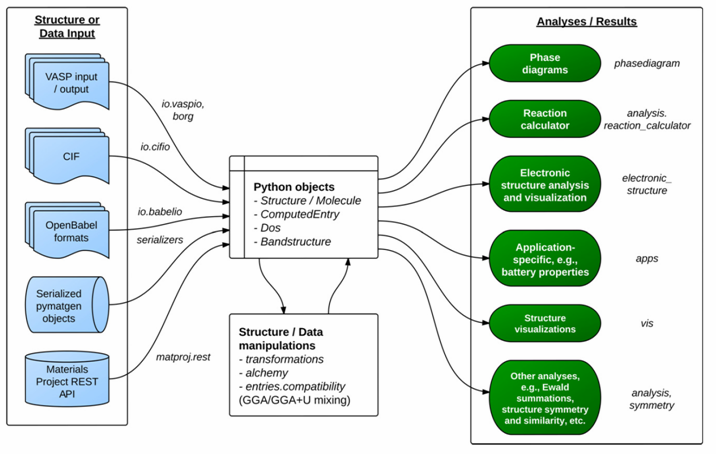
\includegraphics[height=2.3in]{Figures/MP_library.png}
\caption{\fontsize{7.2pt}{4.2pt}\selectfont{\textrm{Overview of a typical workflow for pymatgen.}}}%
\label{Pymatgen_Lib}
\end{figure} 
}

\frame
{
	\frametitle{\textrm{Pymatgen}可展示的材料物性}
\begin{figure}[h!]
\centering
\vspace*{-0.1in}
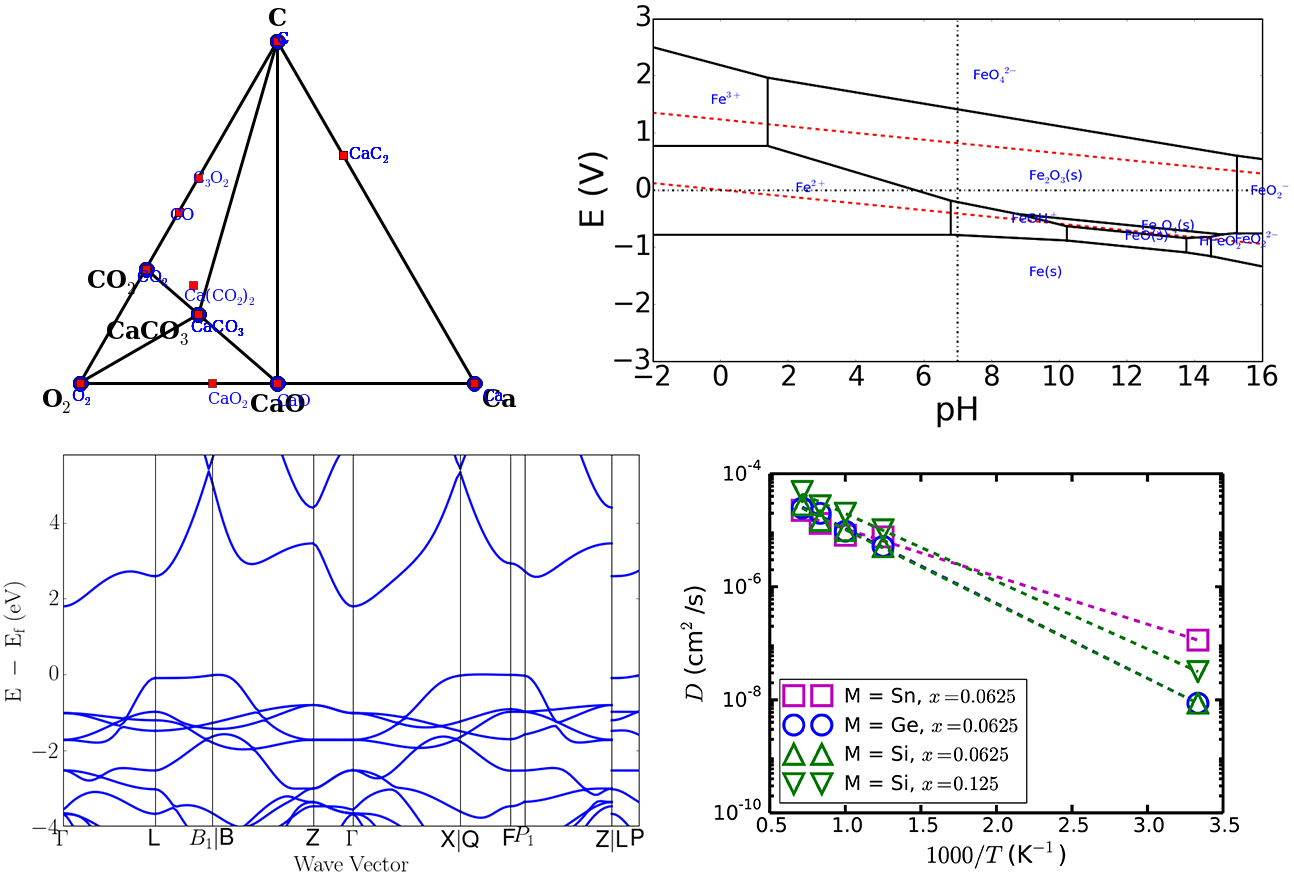
\includegraphics[height=2.3in]{Figures/MP_vision.png}
\caption{\fontsize{5.2pt}{4.2pt}\selectfont{\textrm{Top left: Phase; Top right: Pourbaix diagram from the Materials API. \\Bottom left: Calculated bandstructure plot using pymatgen’s parsing and plotting utilities. Bottom right: Arrhenius plot using pymatgen’s Diffusion~Analyzer.}}}%
\label{Pymatgen_vision}
\end{figure} 
}

\frame
{
	\frametitle{\textrm{FireWorks}的模块结构}
\begin{figure}[h!]
\centering
\vspace*{-0.1in}
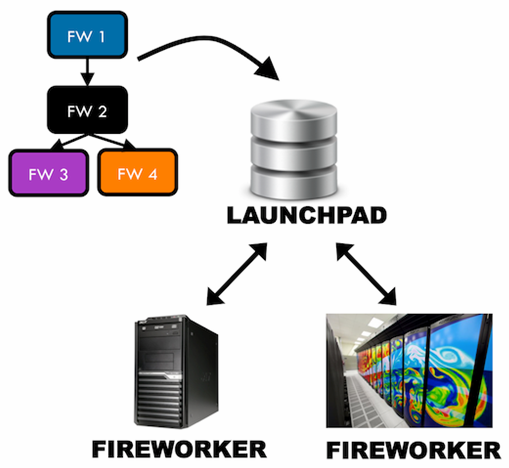
\includegraphics[height=1.8in]{Figures/MP_fireworks.png}
\hskip 1pt
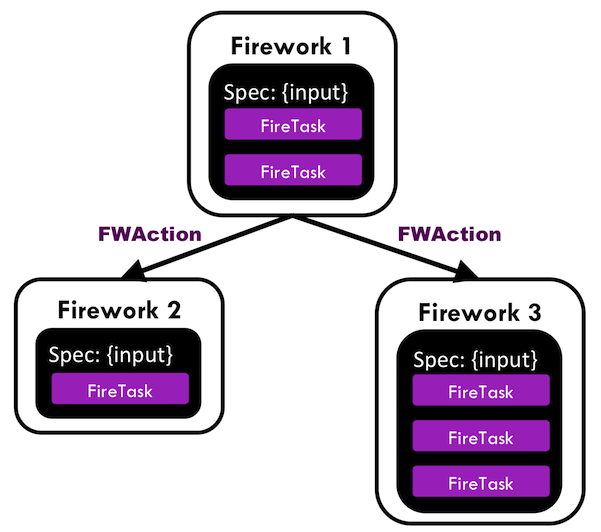
\includegraphics[height=1.8in]{Figures/MP_multiple_fw.png}
\caption{\fontsize{7.2pt}{4.2pt}\selectfont{\textrm{The basic infrastructure of FireWorks.}}}%
\label{FireWorks_FW}
\end{figure} 
}

\frame
{
	\frametitle{\textrm{Custodian}的容错逻辑}
\begin{figure}[h!]
\centering
\vspace*{-0.1in}
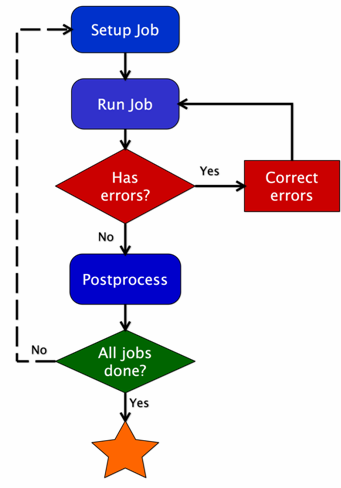
\includegraphics[height=2.3in]{Figures/MP_custodian.png}
\label{Custodian_over}
\caption{\fontsize{7.2pt}{4.2pt}\selectfont{\textrm{Overview of the Custodian workflow.}}}%
\end{figure} 
}

\frame
{
	\frametitle{\textrm{atomate}:~计算流程控制示范}
%		\textcolor{purple}{\textrm{Atomate}}:~:~适合一定复杂程度的\textrm{~VASP~}计算
\begin{figure}[h!]
\centering
\vspace*{-0.1in}
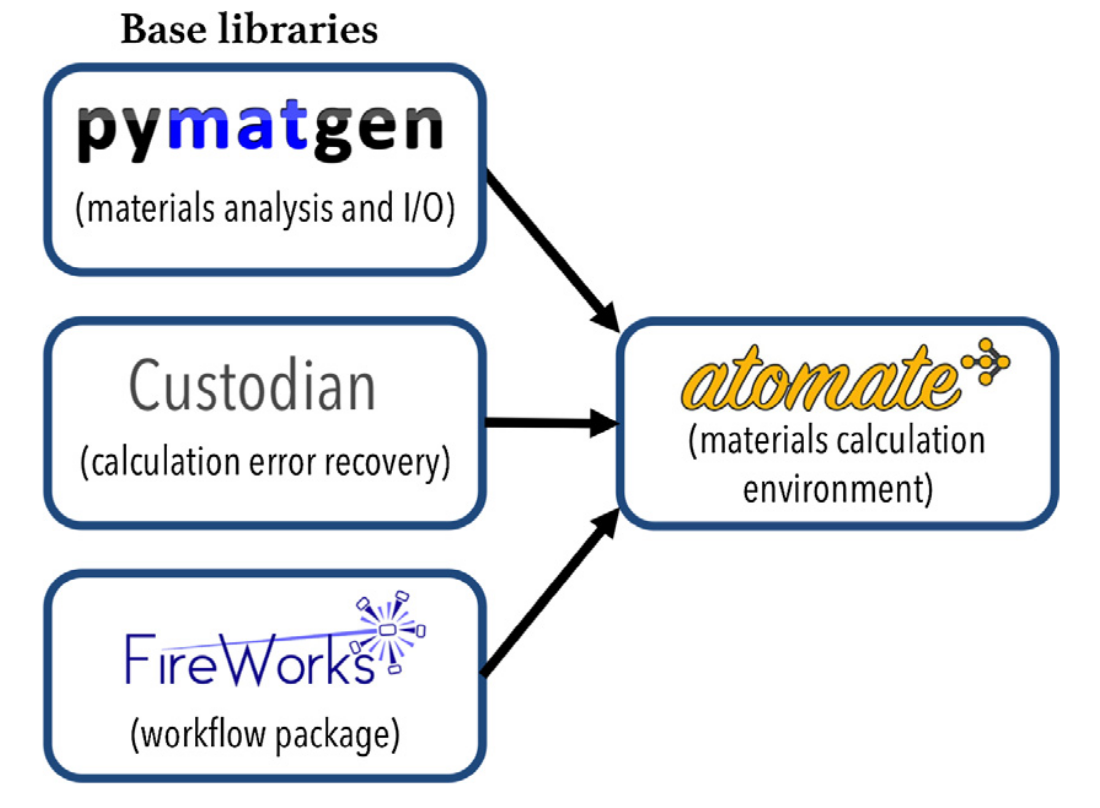
\includegraphics[height=1.3in,width=2.2in,viewport=0 0 820 630,clip]{Figures/Atomate_comp.png}
\vskip 1pt
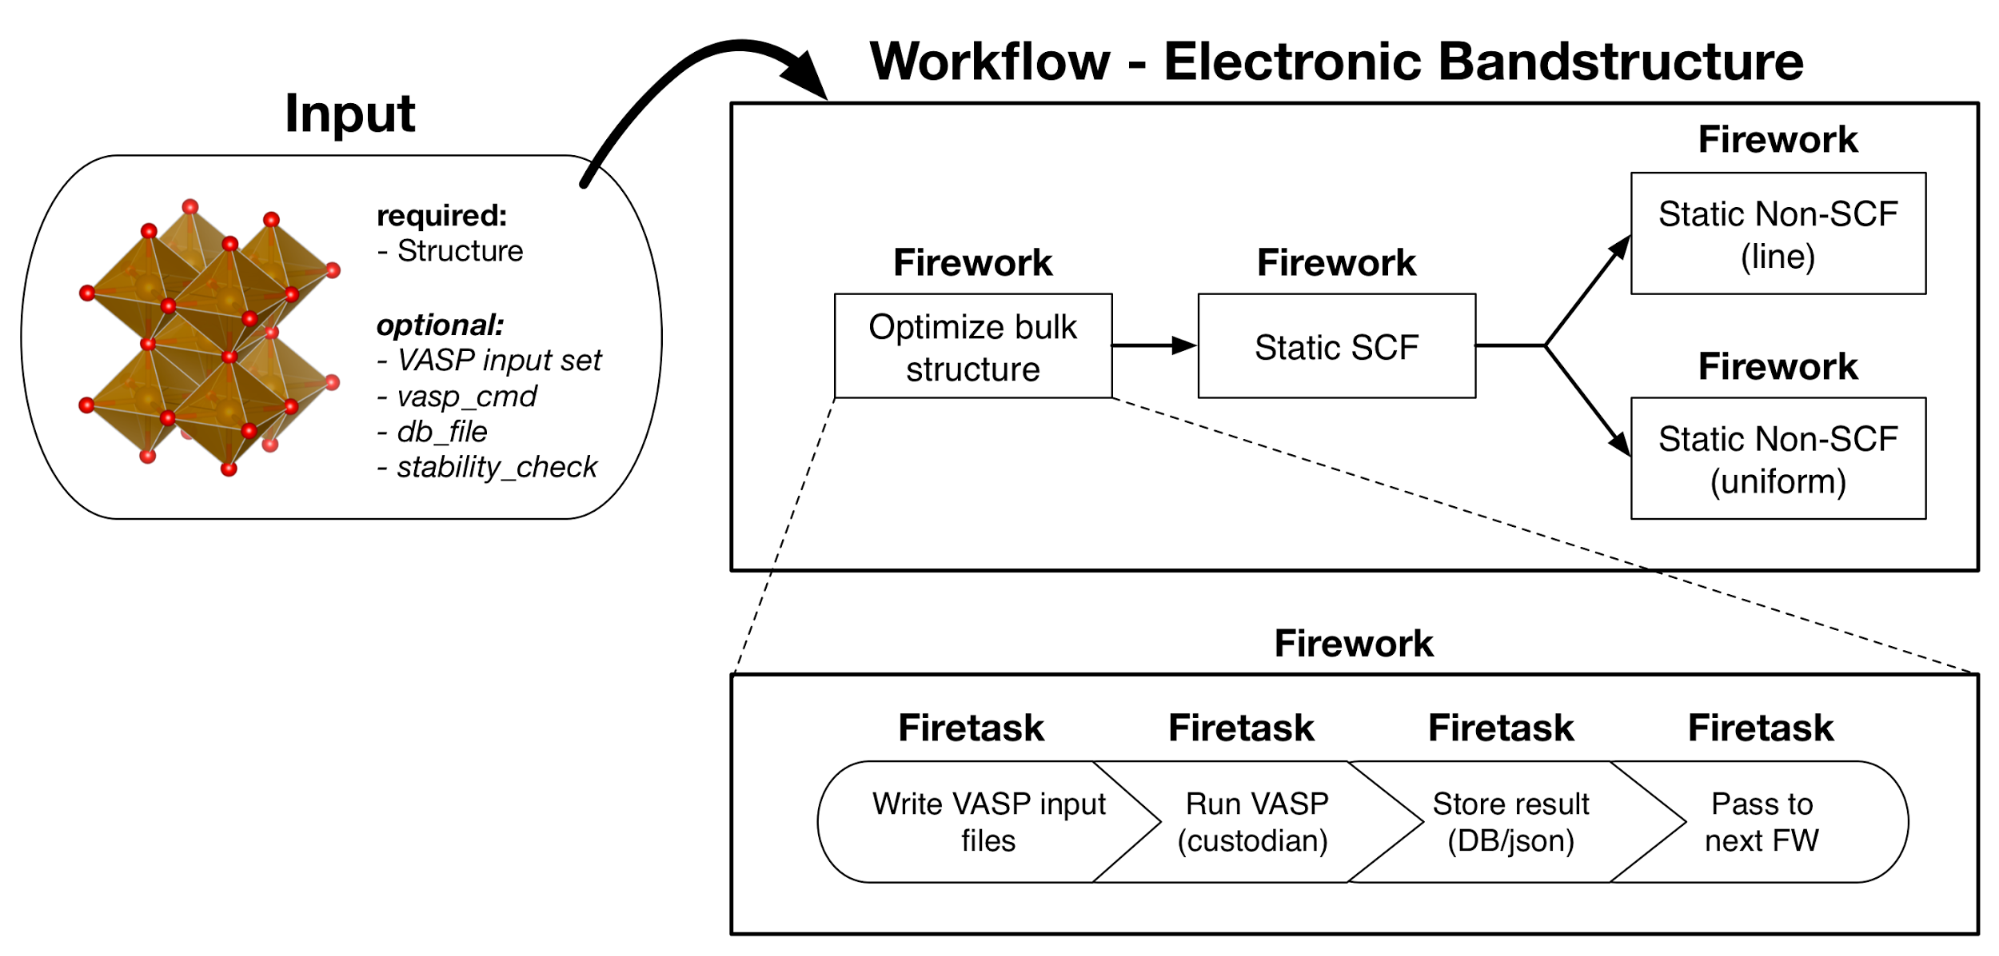
\includegraphics[height=1.5in]{Figures/bandstructure_wf.png}
%\caption{\fontsize{7.2pt}{4.2pt}\selectfont{\textrm{The integrated calculator in ASE (Atomic Simulation Environment).}}}%
\label{Logo_QM-MM}
\end{figure} 
}

\frame
{
	\frametitle{\textrm{ASE}自动流程的设计与管理}
		\textcolor{purple}{\textrm{ASE}}:~模块加载式计算流程控制,更符合复杂多尺度计算场景
		\begin{itemize}
			\item \textcolor{magenta}{灵活的建模功能}
				\begin{enumerate}
    \setlength{\itemsep}{10pt}
					\item 简单堆积:~原子直接组成分子
					\item 理想周期体系(包括一维、二维、三维)
					\item 表面和表面吸附,可指定吸附位
				\end{enumerate}
			\item \textcolor{magenta}{丰富的软件接口}\\
				提供了包括绝大部分第一原理和分子动力学计算软件接口,方便组合实现多尺度计算
			\item \textcolor{magenta}{不依赖软件的优化与动力学模拟}\\
				适合复杂材料物性模拟的优化和多种动力学过程模拟
			\item \textcolor{magenta}{多样化的数据库类型}
		\end{itemize} 
}

\frame
{
\frametitle{\textrm{ASE}特色:~材料结构生成模块}
\begin{figure}[h!]
\centering
\vspace*{-0.27in}
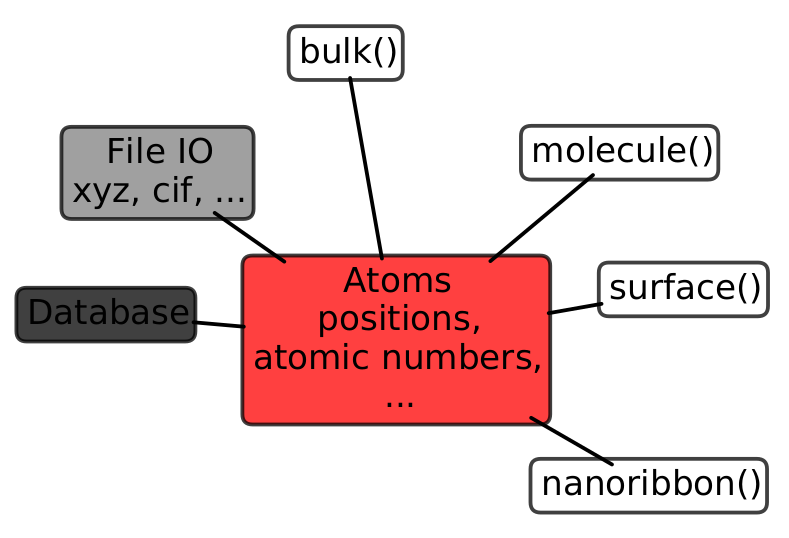
\includegraphics[height=1.3in,width=1.9in,viewport=0 0 820 530,clip]{Figures/ASE_atoms_module.png}
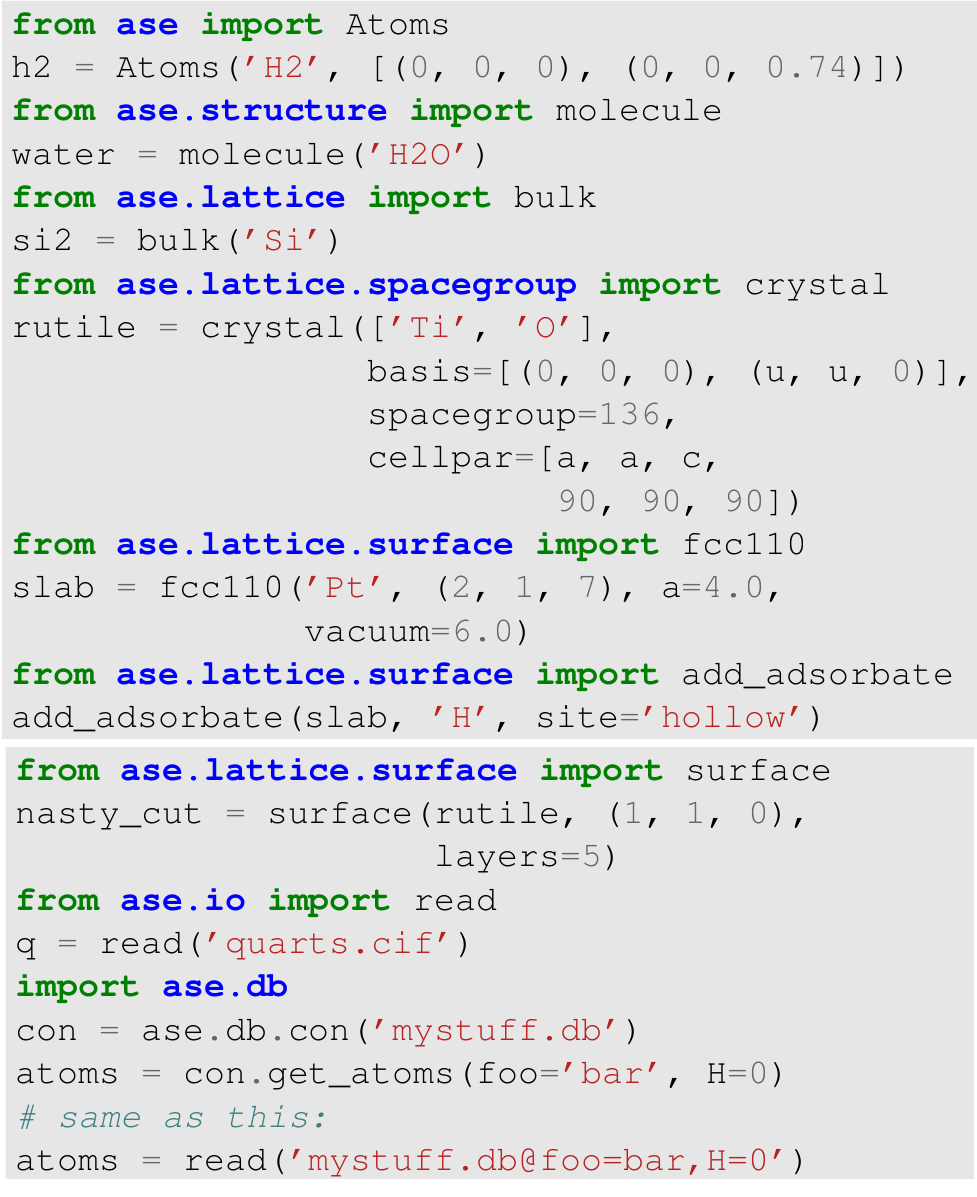
\includegraphics[height=2.9in,width=2.2in,viewport=0 0 970 1200,clip]{Figures/ASE_atoms_module-examples.png}
%\caption{\fontsize{7.2pt}{4.2pt}\selectfont{\textrm{The integrated calculator in ASE (Atomic Simulation Environment).}}}%
\label{Logo_atoms-module}
\end{figure} 
}

\frame
{
\frametitle{\textrm{ASE}特色:~软件接口丰富}
\textcolor{purple}{\textrm{ASE}}:~\textrm{Calculator}模块提供的可选的软件接口
\begin{figure}[h!]
\centering
\vspace*{-0.05in}
%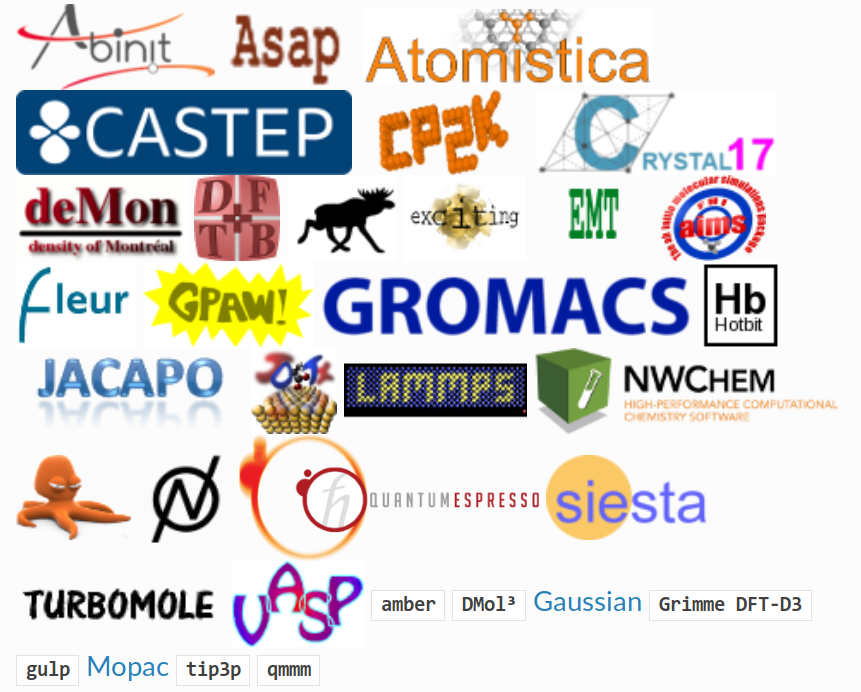
\includegraphics[height=1.0in,width=1.4in,viewport=0 0 638 530,clip]{Figures/ASE_calculator.png}
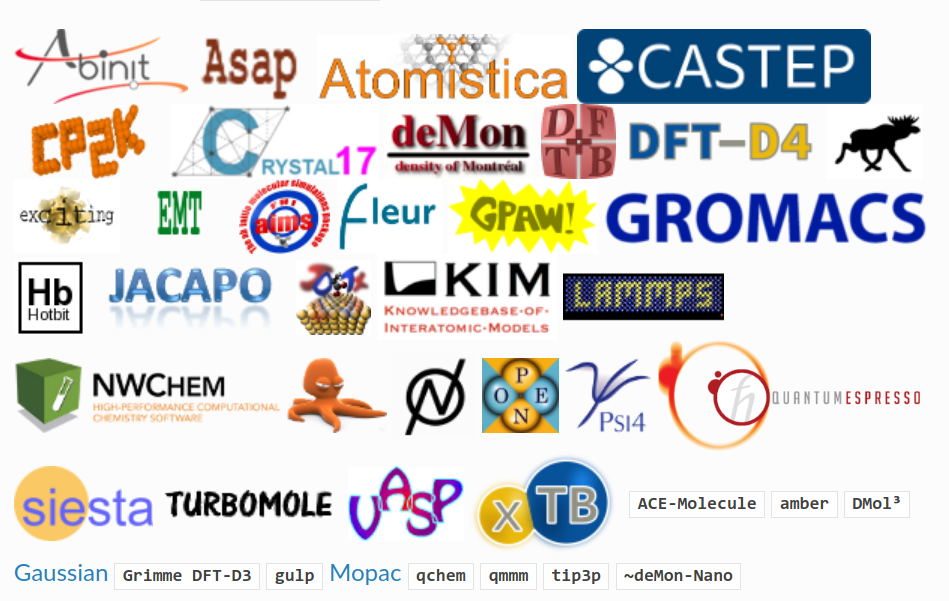
\includegraphics[height=2.0in,width=3.2in,viewport=0 0 940 600,clip]{Figures/ASE_calculator-new.png}
\caption{\fontsize{7.2pt}{4.2pt}\selectfont{\textrm{The integrated calculator in ASE.}}}%
\label{ASE_Calculator}
\end{figure} 
}

\frame
{
\frametitle{\textrm{ASE}特色:~提供多种优化算法模块和数据库}
\begin{figure}[h!]
\centering
\vspace*{-0.21in}
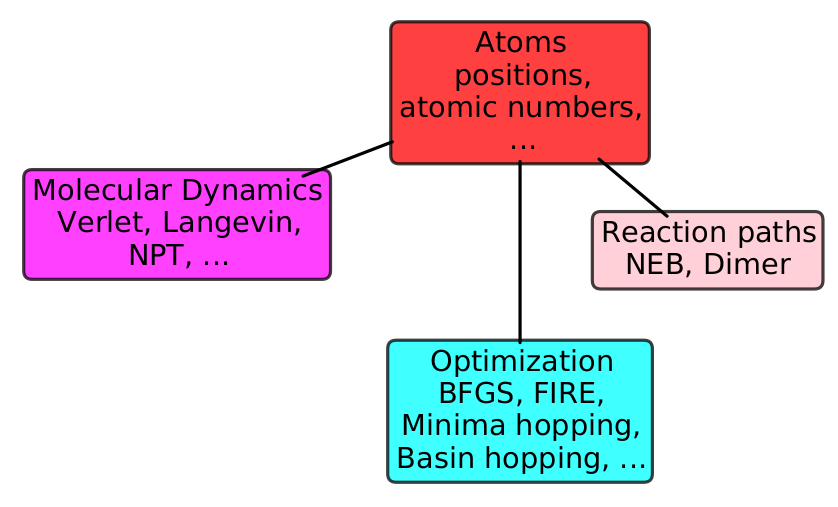
\includegraphics[height=1.3in,width=2.5in,viewport=0 0 838 500,clip]{Figures/ASE_opt_modules.png}
\vskip 1pt
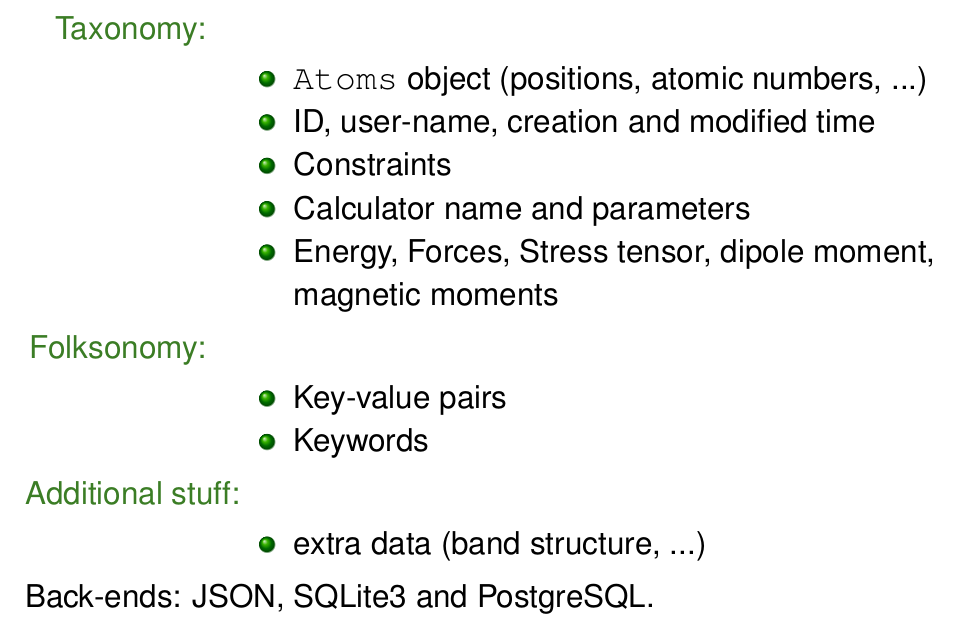
\includegraphics[height=1.7in,width=2.5in,viewport=0 0 938 630,clip]{Figures/ASE_database.png}
\label{ASE_opt-database}
\end{figure} 
}
%\frame
%{
%	\frametitle{\textrm{计算平台的作业自动提交:~基于\textrm{ASE}}}
%\begin{figure}[h!]
%\centering
%\vspace*{-0.2in}
%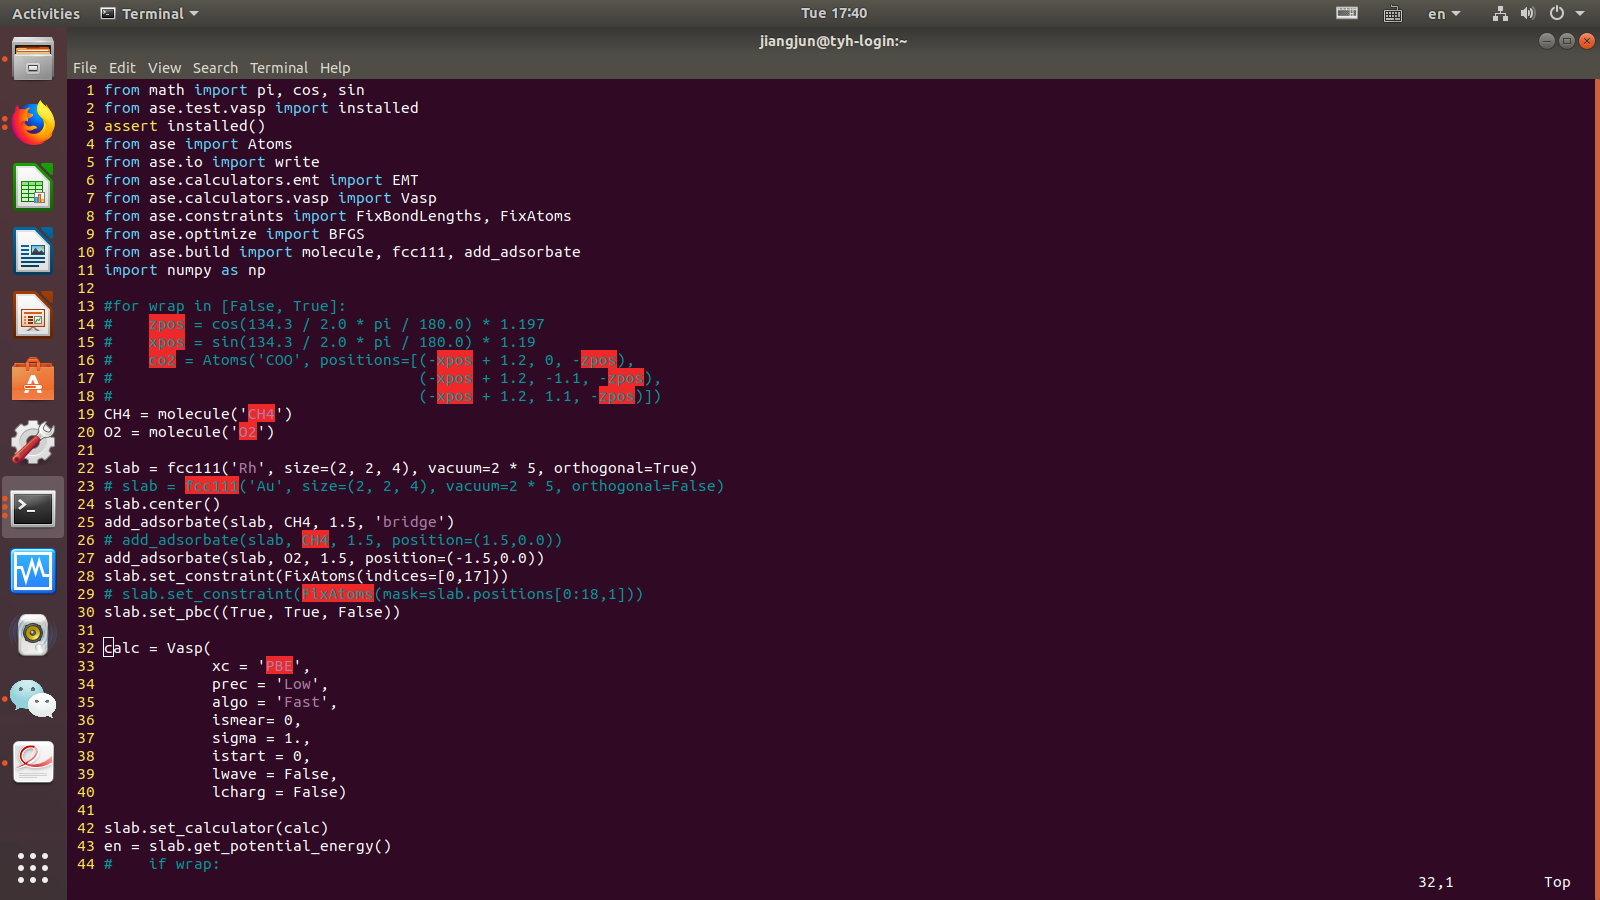
\includegraphics[height=3.1in,width=2.5in,viewport=75 0 725 820,clip]{Figures/ASE_app.png}
%%\caption{\fontsize{7.2pt}{4.2pt}\selectfont{\textrm{The integrated calculator in ASE (Atomic Simulation Environment).}}}%
%\label{ASE_app}
%\end{figure} 
%}

%\frame
%{
%	\frametitle{\textrm{计算平台的结果展示:~基于\textrm{MP}}}
%\begin{figure}[h!]
%\centering
%\vspace*{-0.2in}
%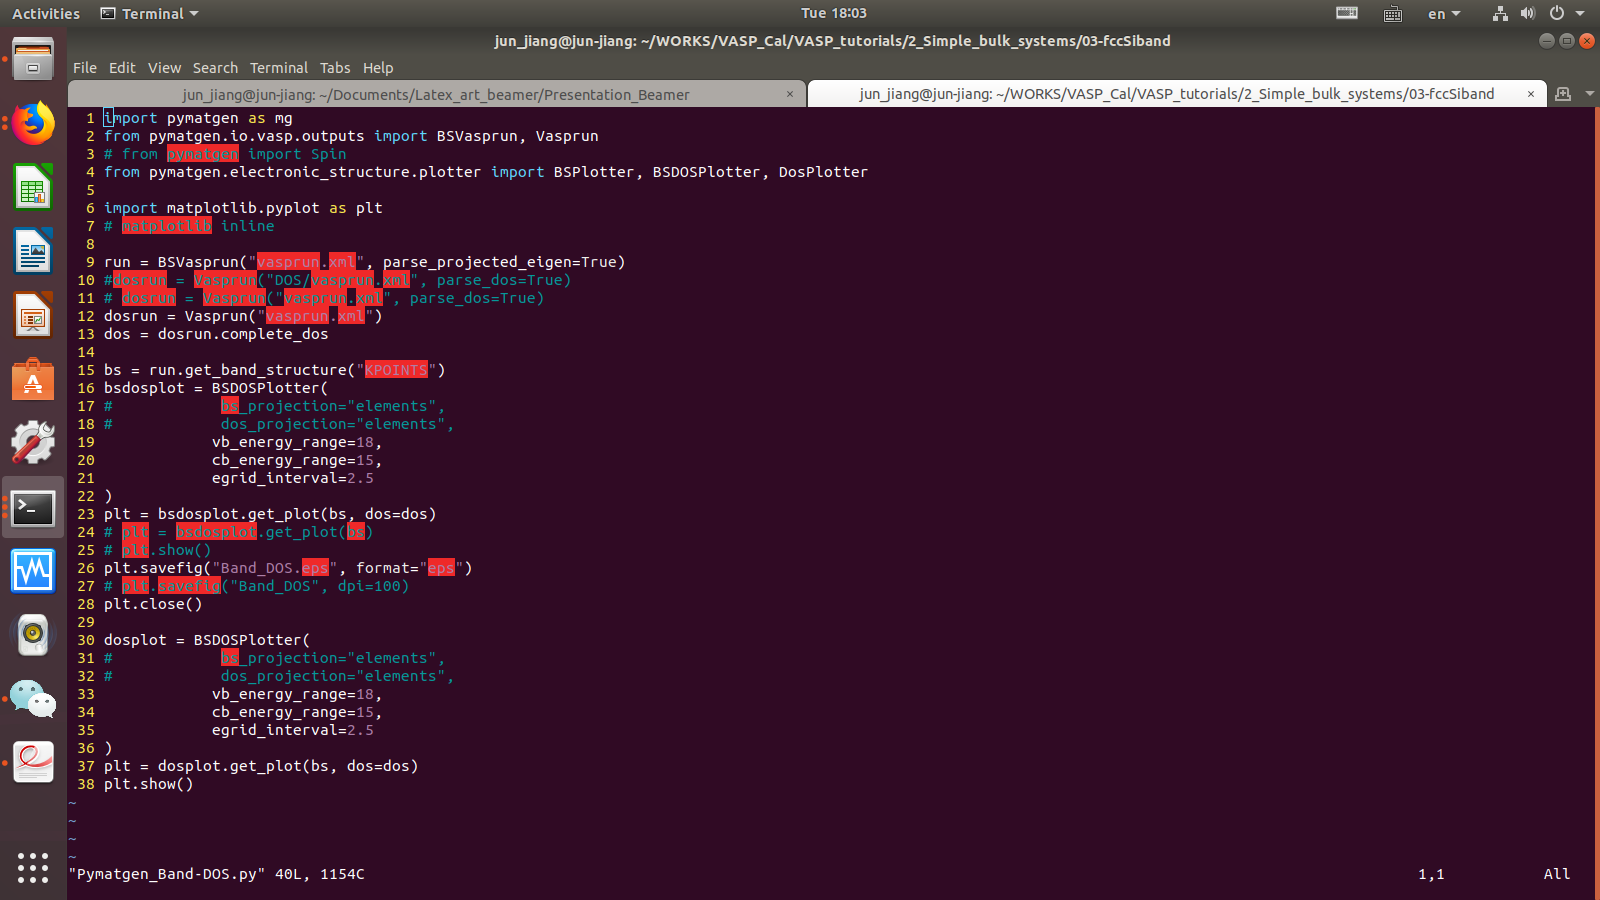
\includegraphics[height=3.1in,width=3.6in,viewport=73 80 880 790,clip]{Figures/Pymatgen_app.png}
%%\caption{\fontsize{7.2pt}{4.2pt}\selectfont{\textrm{The integrated calculator in ASE (Atomic Simulation Environment).}}}%
%\label{Pymatgen_app}
%\end{figure} 
%}
%
\frame
{
	\frametitle{\textrm{计算平台的结果展示:~结合\textrm{MP}与\textrm{ASE}}}
\begin{figure}[h!]
\centering
\vspace*{-0.2in}
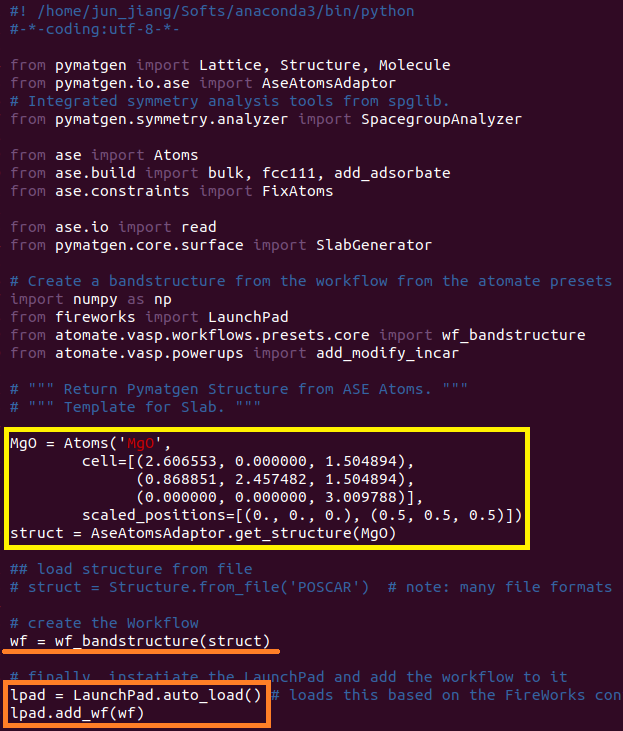
\includegraphics[height=3.0in,width=3.5in,viewport=0 0 600 550,clip]{Figures/Atomate-ASE_MgO.png}
%\caption{\fontsize{7.2pt}{4.2pt}\selectfont{\textrm{The integrated calculator in ASE (Atomic Simulation Environment).}}}%
\label{Atomate-ASE_app}
\end{figure} 
}

\frame
{
	\frametitle{应用示例:~\textrm{MgO:~DOS and Band}}
\begin{figure}[h!]
\centering
\vspace*{-0.2in}
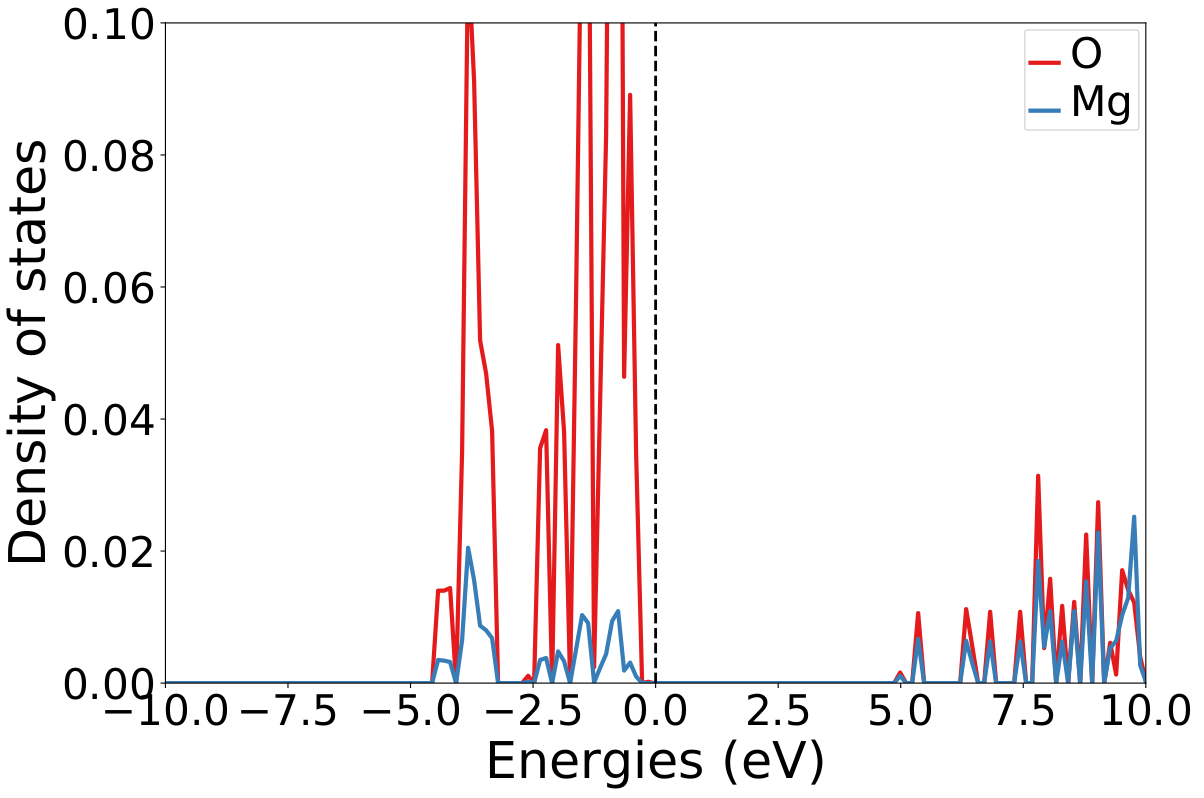
\includegraphics[height=1.5in,width=2.3in,viewport=0 0 900 600,clip]{Figures/Atomate_MgO-DOS.png}
\vskip 1pt
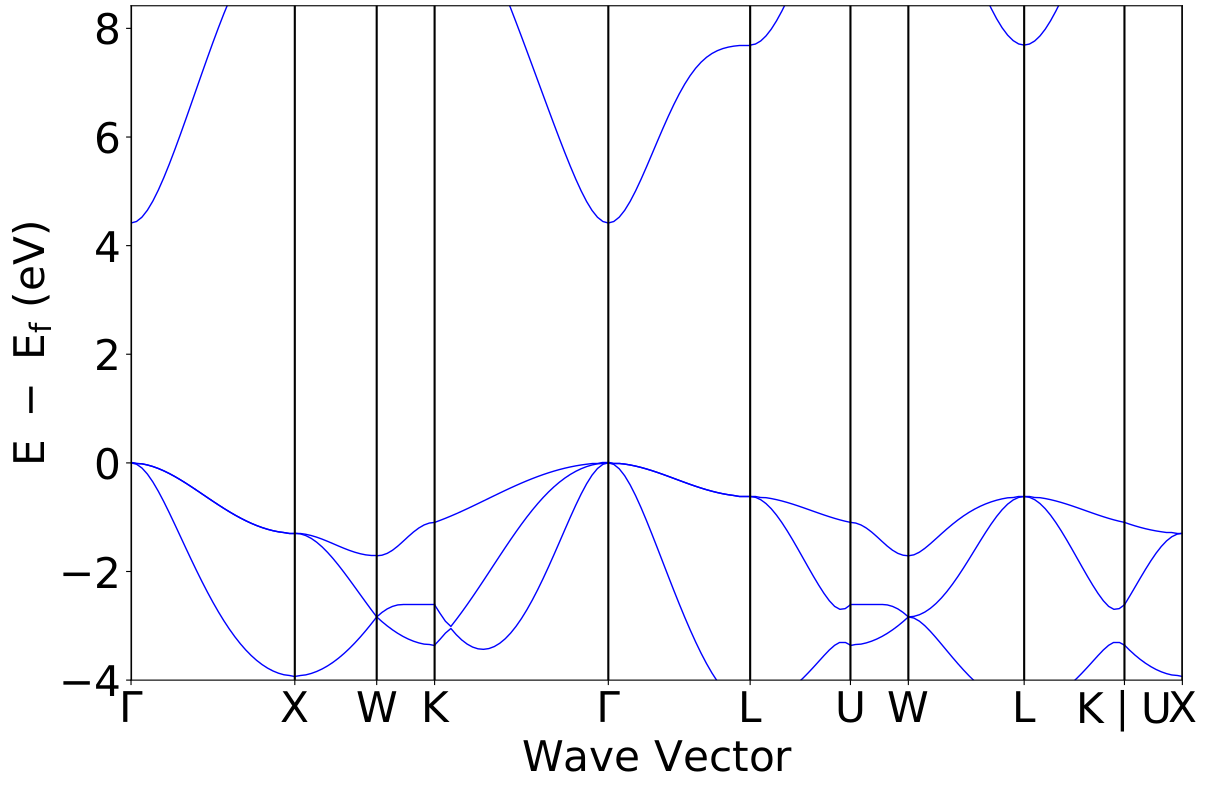
\includegraphics[height=1.5in,width=2.3in,viewport=0 0 900 600,clip]{Figures/Atomate_MgO-Band.png}
%\caption{\fontsize{7.2pt}{4.2pt}\selectfont{\textrm{The integrated calculator in Atomate-ASE.}}}%
\label{Atomate_MgO-DOS}
\end{figure} 
}
%------------------------------------------------------------------------Reference----------------------------------------------------------------------------------------------
%\begin{thebibliography}{99}
%-----------------------------------------------------------------------------------------------------------------------------------------------------------------------%
%\frame
%{
%\frametitle{主要参考文献}
%{\small
%\bibitem{Singh_Book}\textrm{D. J. Singh. \textit{Plane Wave, PseudoPotential and the LAPW method} (Kluwer Academic, Boston,USA, 1994)}					%
%  \nocite{*}																				%
%}
%}
%\end{thebibliography}

\begin{thebibliography}{99}
\frame
{
\frametitle{主要参考文献}
\fontsize{6.5pt}{3.9pt}\selectfont{
	\bibitem{CMS146-319_2018}\textrm{X. Yang, Z. Wang, X. Zhao and H. Liu \textit{Comp. Mater. Sci.}, \textbf{146} (2018), 319}
	\bibitem{url_Matcloud}\textrm{\url{http://matcloud.cnic.cn}}
	\bibitem{CMS58-227_2012}\textrm{S. Curtarolo, W. Setyawan, S. Wang, J. Xue, K. Yang, R. H. Taylor, L. J. Nelson, G. L. Hart, S. Sanvito, M. Buongiorno-Nardelli, N. Mingo and O. Levy \textit{Comp. Mater. Sci.}, \textbf{58} (2012), 227}
	\bibitem{CMS97-209_2015}\textrm{S. P. Ong, S. Cholia, A. Jain, M. Brafman, D. Gunter, G. Ceder and K. A. Persson. \textit{Comp. Mater. Sci.}, \textbf{97} (2015), 209}
	\bibitem{url_QMIP}\textrm{\url{http://www.qmip.org/qmip.org/Welcome.html}}
	\bibitem{JPCL2-2241_2011}\textrm{J. Hachmann, R. Olivares-Amaya, S. Atahan-Evrenk, C. Amador-Bedolla, R. S. S$\acute{a}$nchez-Carrera, A. Gold-Parker, L. Vogt, A. M. Brockway and A. Aspuru-Guzik \textit{J. Phys. Chem. Lett.}, \textbf{2} (2011), 2241}
%	\bibitem{url_Mater_Genome}\textrm{\url{https://www.whitehouse.gov/sites/default/files/microsites/ostp/materials_genome_initiative-final.pdf}}
	\bibitem{CMS49-299_2010}\textrm{W. Setyawan and S. Curtarolo \textit{Comp. Mater. Sci.}, \textbf{49} (2010), 299}
	\bibitem{CMS50-2295_2011}\textrm{A. Jain, G. Hautier, C. J. Moore, S. P. Ong, C. C. Fischer, T. M. Kristin, K. A. Persson and G. Ceder \textit{Comp. Mater. Sci.}, \textbf{50} (2011), 2295}
	\bibitem{unpublished}\textrm{D. Gunter, S. Cholia, A. Jain, M. Kocher, K. Persson, L. Ramakrishnan, S. P. Ong and G. Ceder. \textit{Community Accessible Datastore of High-Throughput Calculations: Experiences from the Materials Project} (unpublished)}
}
\nocite*{}
}
\end{thebibliography}
%{\small
%-----------------------------------------------------------Beamer下不建议使用bib,因为涉及分页--------------------------------------------------------------------------%
%{\small
%\phantomsection\addcontentsline{toc}{section}{Bibliography}	 %直接调用\addcontentsline命令可能导致超链指向不准确,一般需要在之前调用一次\phantomsection命令加以修正	%
%\bibliography{Myref}																			%
%\bibliographystyle{mybib}																		%
%  \nocite{*}																				%
%}

%------------------------------------------------------------------------------------------------------------------------------------------------------------------------------%

%-------------------------------------------------------------------------Thanks------------------------------------------------------------------------------------------------
%\section{致谢}
%\frame
%{
%\frametitle{致$\quad$谢}
%\begin{itemize}
%    \setlength{\itemsep}{20pt}
%  \item 感谢本团队高兴誉、吴泉生、宋红州等各位老师参与的讨论
%  \item 感谢莫所长、宋主任以及软件中心各位老师和同事
%  \item 感谢王崇愚先生的帮助
%\end{itemize}
%}

\logo{}									%不显示logo
\frame
{
\vskip 60 pt
%\hskip 10pt \textcolor{blue}{\Huge 感谢答辩委员会各位老师\,\textrm{!}}\\
\vskip 35 pt
\hskip 60pt \textcolor{blue}{\Huge 谢谢大家\:!}
%\vskip 15 pt
%\hskip 40pt \textcolor{blue}{\Huge \textrm{for your attention\:!}}
}

%-------------------------------------------------------------------------------------------------------------------------------------------------------------------------------

\clearpage
%\end{CJK*}
\end{document}
